\documentclass[12pt,a4paper]{article}
\usepackage{hyperref}
\usepackage{mathtools}
\title{Template for Security-of-Wireless-Networks Reports}
\author{Vasileios Dimitrakis and Niclas Scheuing}

\newcommand{\figurewidth}[0]{.65\textwidth}
\newcommand{\rc}[0]{\emph{Receiver}}
\newcommand{\ap}[0]{\emph{AP}}

\begin{document}
\maketitle
\begin{figure}[h]
	\includegraphics[width=\textwidth]{images/shark_cut.png}
	\caption{Cantenna in the typical Dimitrakis-Scheuing design emphasizing the mediterranean influences.}
	\label{shark}
\end{figure}
\pagebreak
\section{Introduction}
	The objective of this exercise is the creation and the performance evaluation of a high gain
	and directional Wi-Fi antenna. The effectiveness of the antenna will be evaluated in comparison with an omnidirectional and a professional Wi-Fi antenna. The design that we chose to build is a cantenna. Cantenna is a homemade directional waveguide antenna, made out of an open-ended metal can.

\section{Theoretical background of the cantenna}
	The cantenna we built is a cylindrical directional waveguide antenna. This kind of waveguide supports both traverse electric (TE) and traverse magnetic (TM) modes. The traverse modes are a particular electromagnetic field pattern of radiation measured in a plane perpendicular (i.e., transverse) to the propagation direction of the beam. They have a cutoff frequency, below which electromagnetic energy is severely attenuated and above this, the certain mode is excited. An ideal cantenna has only one mode, the dominant one, which is the $TE_{11}$, because our cantenna is a cylindrical waveguide. If the cantenna excites more than one modes, the effectiveness of the antenna will decrease, because the energy of the electromagnetic wave will be spread within different modes. The mode that we do not want to trigger is the $TM_{10}$.
	%TODO: What is this?
	In the following, Figure 1 presents a cantenna setup.
	
	
	\subsection{Cantenna design parameters}
		For our cantenna to work properly, some geometric properties need to be calculated first.
		The cantenna used in this exercise will use the Wi-Fi channel $6$ with central frequency $2.437$GHz and wavelength $12.31$cm.
		
		\subsubsection{Can diameter}
			The cantenna should trigger the dominant mode $TE_{11}$ only. This happens at any frequency higher then the threshold frequency $f_{TE_{11}}$. No other mode is triggered for frequencies below $f_{TE_{11}}$, because waves are attenuated exponentially.
			The second mode is the $TM_{10}$ and if the frequency is greater than the threshold frequency $f_{TM_{10}}$, both the two first modes will be excited.
			We thus deduce that the Wi-Fi frequency $f_{Wi-Fi}$ has to fulfill the following inequality:
			\begin{equation}
				f_{TE_{11}} < f_{Wi-Fi} < f_{TM_{10}}
			\end{equation}.
			
			The formulas for the above two frequencies for the cylindrical waveguide are the following\cite{waveguide}:
			\begin{equation}
				\frac{p_{11} c}{\pi f_{WiFi}} < D < \frac{p_{01}' c}{\pi f_{WiFi}}
			\end{equation}
			%TODO: are the p values correct?
			where $p_{11} = 1.841$ and $p_{01}'= 3.832$ are parameters related to the Bessel function and $c$ the speed of light.
			%TODO: also provide the final values for the equation above
			%TODO: Which limits?
			Therefore the diameter of our cantenna has to be between these limits. 
			%Although these are the theoretical values of the diameter, in real cases, it has to be approximately between 8-11cm, so that the antenna will be effective.
			
		\subsubsection{Position of the copper element: Acts as the monopole} \label{mono:pos}
			Not only that certain modes are triggered, when the electro magnetic wave of the Wi-Fi signal reaches the cantenna. The wave inside the can is also reflected by its bottom. This results in the creation of a static wave.
			The wavelength $\lambda_g$ of the static wave inside of the can is equal to the wavelength of the mode that is triggered. In our case we want to trigger only the dominant mode $TE_{11}$.
			Placing the monopole, we must take into consideration the frequency of this static wave.
			The static wave is a sinusoid, so we know its highest amplitude can be found at a distance of $\frac{\lambda_g}{4}$ from the can bottom.
			Since we know $\lambda = 176.56 mm$ as a property of the $TE_{11}$ mode, we placed the monopole at a distance of $\frac{\lambda_g}{4} = 44.14 mm$ from the can bottom. The monopole is a piece of copper wire placed orthogonally to the can surface pointing inwards.
		
		\subsubsection{Monopole length}
			The monopole antenna is a class of radio antenna consisting of a straight rod-shaped conductor, often mounted perpendicularly over some type of conductive surface, called a plane ground. In our case, we decided to built the most common type of the monopole, which is the quarter-wave monopole. It is also called \emph{Marconi antenna}. This monopole is ideal for our configuration, because it is simple and it has the right dimensions, in order to fit inside the cantenna. The length of the monopole is equal to $\frac{1}{\lambda_{Wi-Fi}}$. Where  $\lambda_{Wi-Fi}$ is the wavelength of the Wi-Fi signal. In the current setup $\lambda_{Wi-Fi} = 123mm$, so the length of the monopole is $30.75mm$.
		
		\subsubsection{Length of the can}
			The length of the can has to be more than $\frac{3}{4}\ {\lambda_g}$. The longer the cantenna is the more directional and effective becomes. In our case, the length of the cantenna is $160mm$, so we expect to be directional.
	
	\subsection{Cantenna theoretical and experimental device dimensions} 
		In \autoref{can:geom}, we present the theoretical design parameters of the cantenna and the actual ones of our setup. Our cantenna satisfies all the design prerequisites and thus, we expect it to work fairly well regarding antenna gain and directivity.

		\begin{table}
			\begin{center}
				\begin{tabular}{r|r|r|r}\
				 & Theoretical value in mm& Actual Values in mm\\
				 \hline 
				 \emph{Can diameter} & 0 & 100.5\\
				 \emph{Monopole position} & 0 & 44.1 \\
				 \emph{Monopole length} & 0 & 30.75\\
				 \emph{Length of the can} & 0 & 162.5\\
				\end{tabular}
			\end{center}
			\caption{Cantenna geometry. Theoretical and actual values.}
			\label{can:geom}
		\end{table}

\section{Setup}	
	
	\subsection{Terminology}
		The machine serving as stationary receiver connected to the cantenna is denoted by \rc. It is the one performing all measurements. The machine used as access point is called \ap. It is moved around and sending traffic to the \rc.
	
	\subsection{Materials}
		The materials and the equipment that were used for the creation and the setup of the antenna are the following: 
		\begin{itemize}
			\item $2$ Notebooks
			\item {\emph{$1$ USB Alfa wireless adapter:} Is the wireless adapter connected to \rc. The antennas are connected to this interface.} 
			\item {\emph{$1$ TP-Link wireless adapter:} Is used by the \ap.}
			\item {\emph{$1$ Pigtail cable:} Is used to connect the cantenna with the USB Alfa wireless adapter.}
			\item {\emph{$1$ female N-connector}}
			\item {\emph{$1$ piece of copper wire:} Is used as the active element, the monopole, that radiates the waves}
			\item {\emph{$1$ cylindrical can:} Plays the role of the Wi-fi antenna.} 
			\item \emph{ifconfig}: Is used to configure the network interfaces.
			\item \emph{iwconfig}: Is used to configure the \emph{wireless} network interfaces.
			\item \emph{iperf}: Network testing tool for creating data streams and measuring throughput.
			\item \emph{iptraf}: Monitoring network interface throughput.
			\item \emph{hostapd}: Is a user space deamon for Access Point and authentication servers.
		\end{itemize}
	
	\subsection{Setting up the experiment}
		\paragraph{Wi-Fi channel}: We used Wi-Fi channel $6$.
		\paragraph{Distance meassurement} We placed markers on the ground(see \autoref{marks}) at the distances of 1m, 10m, 20m, 40m, 60m, 80m, 100m. To measure the distance we used GPS and counting steps, which resulted in a maximum difference of less than 2m.
		\begin{figure}
			\includegraphics[width=\textwidth]{images/marks_cut.png}
			\caption{Markers placed on the side of the road for the distance measurements.}
			\label{marks}
		\end{figure}
		
		\paragraph{Cantenna mounting} To keep the antennas stable in position and angle, we mounted them on a microphone stand. See \autoref{setup}
		\begin{figure}
			\begin{centering}
				\includegraphics[width=.7\textwidth]{images/setup_cut.png}
				\caption{All three antennas are stable in position and direction.}
				\label{setup}
			\end{centering}
		\end{figure}
		\paragraph{Access Point} The access point run on the \ap machine using \emph{hostapd}

\section{Results}
	This section is divided in two different subsections: The one is the gain measurements and the other is the directionality measurements. 
	
	\subsection{Gain measurements}
		In this phase of our experiment, we will compare the way that the signal strength changes increasing the distance of the AP and the antenna under test (client). This experiment will be executed for three different antennas: an omnidirectional antenna, a professional cantenna and our cantenna. In order to be the measurements accurate, they have to be taken in an open area field. For this reason, we chose the place, that is depicted in the following pictures, in order to avoid environmental effects, such as reflections by buildings, scattering by moving objects.
	
	\subsection{Directionality measurements}
		The second phase of the experiment evaluates the directionality of each of the above antennas. All the measurements for the three antennas will be taken in $20$m distance from the Access Point. The starting point of the measurements will be considered the one with $^{\circ}$. Every next measurement will be taken every $20^{\circ}$.

	\subsection{Maximum distance measurements}
		\begin{figure}
			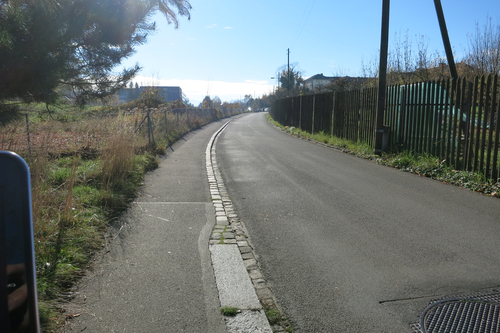
\includegraphics[width=\textwidth]{images/distance.JPG}
			\caption{title}
			\label{distance}
		\end{figure}
		
		\begin{figure}
			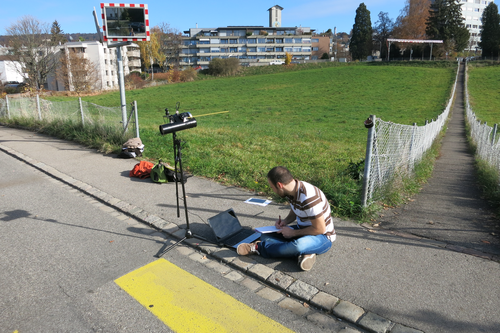
\includegraphics[width=\textwidth]{images/cool.JPG}
			\caption{title}
			\label{cool}
		\end{figure}




\section{Analysis}

\section{References}
\bibliographystyle{plain}
\bibliography{bibliography}


\section{Appendix}
\pagestyle{empty}
\begin{figure}\begin{center}
	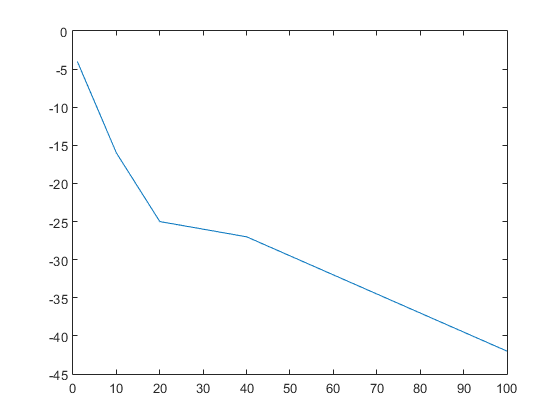
\includegraphics[width=\figurewidth]{plots/can_p.png}
	\caption{Our cantenna. Measured signal strength depending on the distance}
	\label{img:dist:pow:can}

	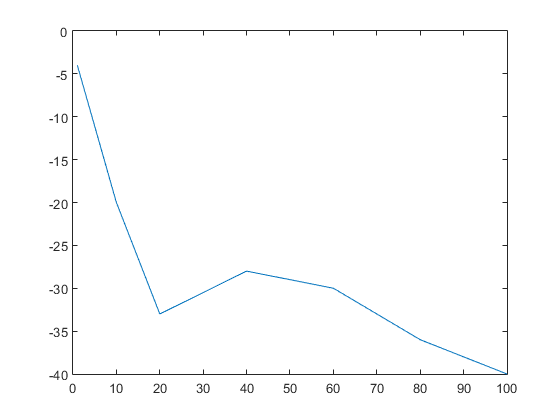
\includegraphics[width=\figurewidth]{plots/prof_p.png}
	\caption{Professional cantenna. Measured signal strength depending on the distance}
	\label{img:dist:pow:prof}

	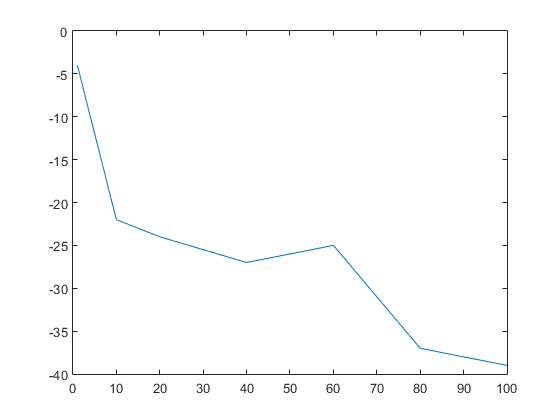
\includegraphics[width=\figurewidth]{plots/omni_p.png}
	\caption{Omni-directional cantenna. Measured signal strength depending on the distance}
	\label{img:dist:pow:omni}
\end{center}\end{figure}

%distance bandwidth
\begin{figure}\begin{center}
	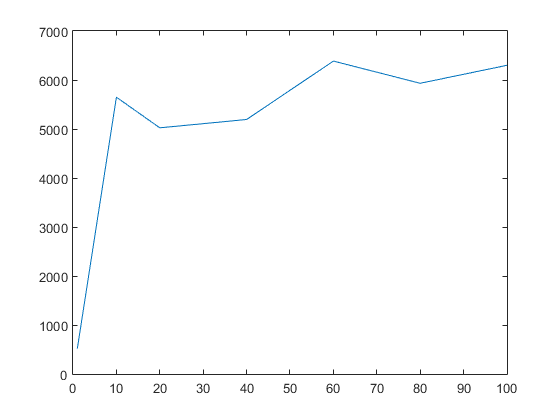
\includegraphics[width=\figurewidth]{plots/can_b.png}
	\caption{Our cantenna. Measured bandwidth depending on the distance}
	\label{img:dist:band:can}

	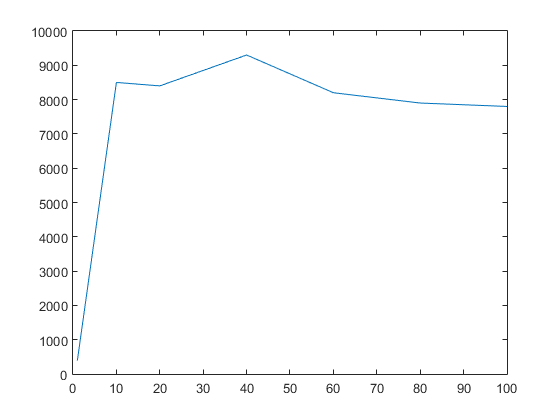
\includegraphics[width=\figurewidth]{plots/prof_b.png}
	\caption{Professional cantenna. Measured bandwidth depending on the distance}
	\label{img:dist:band:prof}


	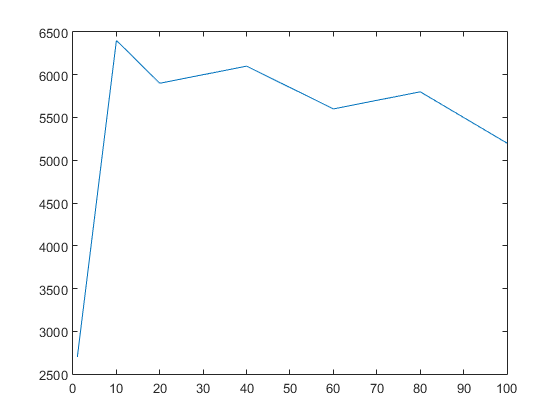
\includegraphics[width=\figurewidth]{plots/omni_b.png}
	\caption{Omni-directional cantenna. Measured 1bandwidth depending on the distance}
	\label{img:dist:band:omni}
\end{center}\end{figure}

%angular pow
\begin{figure}\begin{center}
	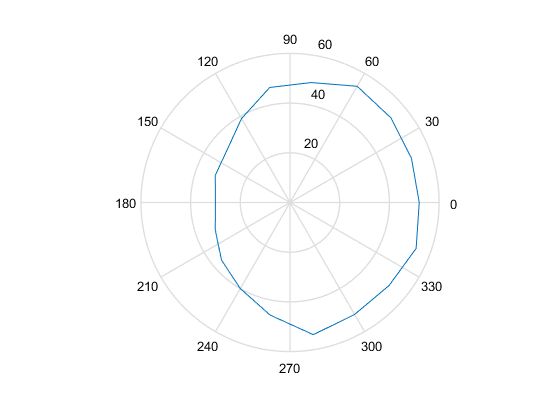
\includegraphics[width=\figurewidth]{plots/polar_can_p.png}
	\caption{Our cantenna. Measured signal strength depending on the angle}
	\label{img:ang:pow:can}

	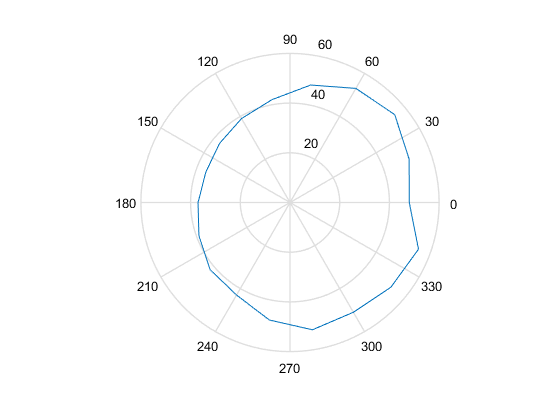
\includegraphics[width=\figurewidth]{plots/polar_prof_p.png}
	\caption{Professional cantenna. Measured signal strength depending on the angle}
	\label{img:ang:pow:prof}

	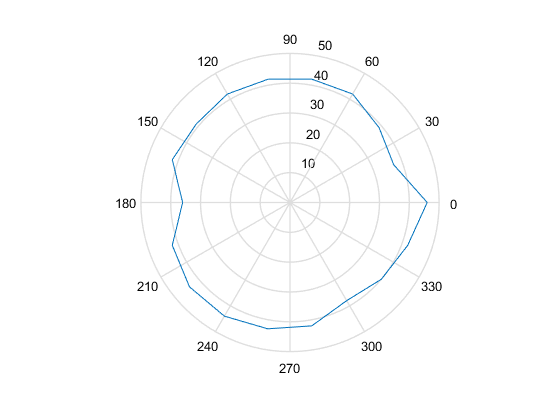
\includegraphics[width=\figurewidth]{plots/polar_omni_p.png}
	\caption{Omni-directional cantenna. Measured signal strength depending on the angle}
	\label{img:ang:pow:omni}
\end{center}\end{figure}

%angular bandwidth
\begin{figure}\begin{center}
	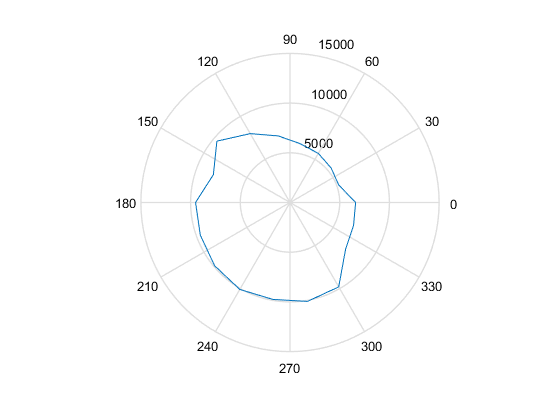
\includegraphics[width=\figurewidth]{plots/polar_can_b.png}
	\caption{Our cantenna. Measured bandwidth depending on the angle}
	\label{img:ang:band:can}

	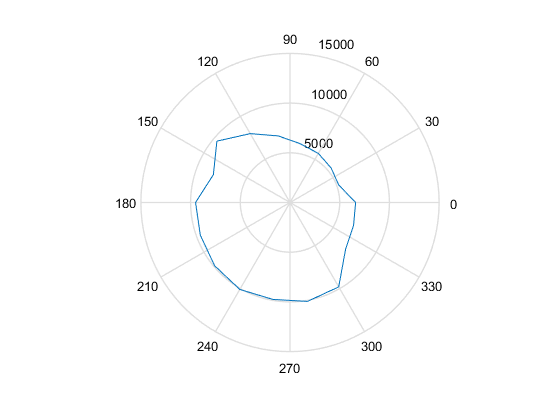
\includegraphics[width=\figurewidth]{plots/polar_prof_b.png}
	\caption{Professional cantenna. Measured bandwidth depending on the angle}
	\label{img:ang:band:prof}

	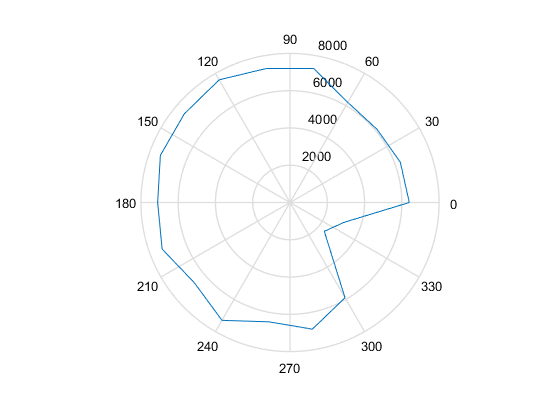
\includegraphics[width=\figurewidth]{plots/polar_omni_b.png}
	\caption{Omni-directional cantenna. Measured bandwidth depending on the angle}
	\label{img:ang:band:omni}
\end{center}\end{figure}

%cantenna

\begin{table}
	\begin{center}
		\begin{tabular}{r|r|r}\
		 Distance in $m$ & signal strength in $dBm$ & transfer rate in $Kib/s$\\
		 \hline 
		 1 & -4 & 520\\
		 10 & -16 & 5649\\
		 20 & -25 & 5024\\
		 40 & -27 & 5194\\
		 60 & -32 & 6386\\
		 80 & -37 & 5933\\
		 100 & -42 & 6300\\
		\end{tabular}
	\end{center}
	\caption{Our cantenna. Measured signal strength and bandwidth depending on the distance}
	\label{dist:can}
\end{table}

%prof cantenna
\begin{table}
	\begin{center}
		\begin{tabular}{r|r|r}\
			Distance in $m$ & signal strength in $dBm$ & transfer rate in $Kib/s$\\
			\hline 
			1 & -4 & 389\\
			10 & -20 & 8500\\
			20 & -33 & 8400\\
			40 & -28 & 9300\\
			60 & -30 & 8200\\
			80 & -36 & 7900\\
			100 & -40 & 7800\\
		\end{tabular}
	\end{center}
	\caption{Professional cantenna. Measured signal strength and bandwidth depending on the distance}
	\label{dist:prof}
\end{table}

%onmi cantenna
\begin{table}
	\begin{center}
		\begin{tabular}{r|r|r}\
			Distance in $m$ & signal strength in $dBm$ & transfer rate in $Kib/s$\\
			\hline 
			1 & -4 & 2700\\
			10 & -22 & 6400\\
			20 & -24 & 5900\\
			40 & -27 & 6100\\
			60 & -25 & 5600\\
			80 & -37 & 5800\\
			100 & -39 & 5200\\
		\end{tabular}
	\end{center}
	\caption{Omni-directional antenna. Measured signal strength and bandwidth depending on the distance}
	\label{dist:omni}
\end{table}


% cantenna angular
\begin{table}
	\begin{center}
		\begin{tabular}{r|r|r}\
			Angle in degrees $m$ & signal strength in $dBm$ & transfer rate in $Kib/s$\\
			\hline 
			0 & -30 & 6600\\
			20 & -32 & 5200\\
			40 & -36 & 5400\\
			60 & -40 & 5700\\
			80 & -46 & 6000\\
			100 & -54 & 6800\\
			120 & -52 & 8000\\
			140 & -52 & 9600\\
			160 & -54 & 8200\\
			180 & -52 & 9500\\
			200 & -52 & 9600\\
			220 & -53 & 9900\\
			240 & -54 & 10100\\
			260 & -49 & 9900\\
			280 & -47 & 10100\\
			300 & -39 & 9800\\
			320 & -33 & 7300\\
			340 & -32 & 6800\\
		\end{tabular}
	\end{center}
	\caption{Our cantenna. Measured signal strength and bandwidth depending on the angle}
	\label{ang:can}
\end{table}

% prof cantenna angular
\begin{table}
	\begin{center}
		\begin{tabular}{r|r|r}\
			Angle in degrees $m$ & signal strength in $dBm$ & transfer rate in $Kib/s$\\
			\hline 
			0 & -37 & 7900\\
			20 & -39 & 7100\\
			40 & -42 & 7200\\
			60 & -43 & 7300\\
			80 & -48 & 8200\\
			100 & -52 & 9300\\
			120 & -51 & 9900\\
			140 & -53 & 9600\\
			160 & -55 & 9400\\
			180 & -48 & 10300\\
			200 & -51 & 10300\\
			220 & -55 & 9200\\
			240 & -53 & 9800\\
			260 & -48 & 10300\\
			280 & -42 & 10300\\
			300 & -39 & 10300\\
			320 & -37 & 7900\\
			340 & -36 & 7700\\
		\end{tabular}
	\end{center}
	\caption{Pofessional cantenna. Measured signal strength and bandwidth depending on the angle}
	\label{ang:prof}
\end{table}

% omni angular
\begin{table}
	\begin{center}
		\begin{tabular}{r|r|r}\
			Angle in degrees $m$ & signal strength in $dBm$ & transfer rate in $Kib/s$\\
			\hline 
			0 & -36 & 6400\\
			20 & -42 & 6300\\
			40 & -44 & 6100\\
			60 & -44 & 6200\\
			80 & -43 & 7300\\
			100 & -42 & 7300\\
			120 & -38 & 7600\\
			140 & -40 & 7400\\
			160 & -42 & 7400\\
			180 & -46 & 7100\\
			200 & -37 & 7300\\
			220 & -39 & 6700\\
			240 & -42 & 7300\\
			260 & -42 & 6500\\
			280 & -42 & 6900\\
			300 & -42 & 5900\\
			320 & -41 & 2400\\
			340 & -42 & 3100\\
		\end{tabular}
	\end{center}
	\caption{Omni-directional antenna. Measured signal strength and bandwidth depending on the angle}
	\label{ang:omni}
\end{table}




\end{document}